% This is "bach-ref-2009.tex" Updated january 29th 2010.
% This file should be compiled with "sig-alternate-fixed.cls" January 2010.
% It is based on the ACM style "sig-alternate.cls"
% -----------------------------------------------------------------------
% This example file demonstrates the use of the 'sig-alternate-fixed.cls'
% V2.5 LaTeX2e document class file. It is for those submitting
% articles to the Twente Student Conference on IT. Both this file as the 
% document class file are based upon ACM documents.
%
% ------------------------------------------------------------------------
% This .tex file (and associated .cls) produces:
%       1) The Permission Statement
%       2) The Conference (location) Info information
%       3) The Copyright Line TSConIT
%       4) NO headers and/or footers
%
%
% Using 'sig-alternate.cls' you have control, however, from within
% the source .tex file, over both the CopyrightYear
% (defaulted to 200X) and the ACM Copyright Data
% (defaulted to X-XXXXX-XX-X/XX/XX).
% e.g.
% \CopyrightYear{2007} will cause 2007 to appear in the copyright line.
% \crdata{0-12345-67-8/90/12} will cause 0-12345-67-8/90/12 to appear in the copyright line.
%
% ------------------------------------------------------------------------
% This .tex source is an example which *does* use
% the .bib file (from which the .bbl file % is produced).
% REMEMBER HOWEVER: After having produced the .bbl file,
% and prior to final submission, you *NEED* to 'insert'
% your .bbl file into your source .tex file so as to provide
% ONE 'self-contained' source file.
%

% refers to the cls file being used
\documentclass{sig-alternate-br}
\usepackage[hyphens]{url}
\usepackage[table]{xcolor}% http://ctan.org/pkg/xcolor
% set urls to italics instead of bold
\def\UrlFont{\em}

% balance the columns on the last page
\usepackage{balance}

\begin{document}
%
% --- Author Metadata here --- DO NOT REMOVE OR CHANGE 
\conferenceinfo{31$^{st}$ Twente Student Conference on IT}{Jul. 5$^{th}$, 2019, Enschede, The Netherlands.}
\CopyrightYear{2019} % Allows default copyright year (200X) to be over-ridden - IF NEED BE.
%\crdata{0-12345-67-8/90/01}  % Allows default copyright data (0-89791-88-6/97/05) to be over-ridden - IF NEED BE.
% --- End of Author Metadata ---

\title{Hacking the router: characterizing attacks targeting low-cost routers using a honeypot router}
% In Bachelor Referaat at University of Twente the use of a subtitle is discouraged.
% \subtitle{[Instructions]}

%
% You need the command \numberofauthors to handle the 'placement
% and alignment' of the authors beneath the title.
%
% For aesthetic reasons, we recommend 'three authors at a time'
% i.e. three 'name/affiliation blocks' be placed beneath the title.
%
% NOTE: You are NOT restricted in how many 'rows' of
% "name/affiliations" may appear. We just ask that you restrict
% the number of 'columns' to three.
%
% Because of the available 'opening page real-estate'
% we ask you to refrain from putting more than six authors
% (two rows with three columns) beneath the article title.
% More than six makes the first-page appear very cluttered indeed.
%
% Use the \alignauthor commands to handle the names
% and affiliations for an 'aesthetic maximum' of six authors.
% Add names, affiliations, addresses for
% the seventh etc. author(s) as the argument for the
% \additionalauthors command.
% These 'additional authors' will be output/set for you
% without further effort on your part as the last section in
% the body of your article BEFORE References or any Appendices.

\numberofauthors{3} %  in this sample file, there are a *total*
% of EIGHT authors. SIX appear on the 'first-page' (for formatting
% reasons) and the remaining two appear in the \additionalauthors section.
%
\author{
% You can go ahead and credit any number of authors here,
% e.g. one 'row of three' or two rows (consisting of one row of three
% and a second row of one, two or three).
%
% The command \alignauthor (no curly braces needed) should
% precede each author name, affiliation/snail-mail address and
% e-mail address. Additionally, tag each line of
% affiliation/address with \affaddr, and tag the
% e-mail address with \email.
%
% 1st. author
\alignauthor
Christian Scholten\\
       \affaddr{University of Twente}\\
       \affaddr{P.O. Box 217, 7500AE Enschede}\\
       \affaddr{The Netherlands}\\
       \email{c.p.b.scholten@student.utwente.nl}
}
% There's nothing stopping you putting the seventh, eighth, etc.
% author on the opening page (as the 'third row') but we ask,
% for aesthetic reasons that you place these 'additional authors'
% in the \additional authors block, viz.
% \additionalauthors{Additional authors: John Smith (The
% Th{\o}rv{\"a}ld Group, email: {\texttt{jsmith@affiliation.org}})
% and Julius P.~Kumquat (The Kumquat Consortium, email:
% {\texttt{jpkumquat@consortium.net}}).}
% \date{30 July 1999}
% Just remember to make sure that the TOTAL number of authors
% is the number that will appear on the first page PLUS the
% number that will appear in the \additionalauthors section.

\maketitle
\begin{abstract}
In this paper hacker attacks against low-cost routers have been investigated with the goal to get a better understanding of the intents of hackers and to find ways to improve defense mechanisms for these devices. This has been achieved by characterizing and analyzing real hacker attacks performed against a honeypot router device in a cloud environment. RouterOS from MikroTik has been run in a cloud environment as a honeypot to capture hacker attacks. Using this environment, multiple attacks have been discovered, including traffic related to CVE-2018-14847, which contributed 71.1\% of all traffic on MikroTik specific port 8291. Some successful DNS redirection attempts were discovered and attacks were received that managed to reboot the honeypot router by sending one or multiple RST packets.
\end{abstract}

% A category with the (minimum) three required fields (NOT USED in Bachelor Referaat)
% \category{H.4}{Information Systems Applications}{Miscellaneous}
%A category including the fourth, optional field follows...
% \category{D.2.8}{Software Engineering}{Metrics}[complexity
% measures, performance measures]

\keywords{low-cost routers, MikroTik, RouterOS, honeypot, security, vulnerabilities, hacker attacks}

\section{Introduction}
Low cost routers have been a popular infrastructure device in underdevelopment countries, where they are used for expanding internet coverage in remote places. Low cost routers are cheap router devices which can be used as a home router or as a local area router with more advanced routing features such as the Border Gateway Protocol (BGP). These devices have been a popular target hackers with these attacks becoming more and more popular, with lots of regular news coverage of these devices actively being exploited. For example, the FBI discovered that hundreds of thousands of home routers were vulnerable against attacks from Russian hackers \cite{FBIRus:REUTERS:2018}.

There are many different vendors providing these low cost router devices. Some of the popular vendors include Huawei, TP-Link, NetGear and MikroTik. With over 1.6 million devices publicly visible \cite{MIKROTIK:SHODAN:2019}, MikroTik is a popular manufacturer of these low cost routers. In recent years, multiple vulnerabilities for MikroTik routers with a CVSS \cite{CVSS} score of 7 or higher were discovered \cite{CVELIST}. These vulnerabilities have been a source for many attacks, one of which included two hundred thousand compromised MikroTik routers being used for mining cryptocurrency \cite{MikroTikCryptoHack:PCMAG:2018}. To protect systems and improve the security of the internet, it is important to characterize the attacks to such devices. By doing that, we can understand the intends of the hackers and set proper defenses. 

In this paper, attacks on low cost routers will be characterized by using a honeypot router device in a cloud environment to capture real hacker attacks. A honeypot is a computer system intended to mimic targets of cyber attacks. These honeypots can be used to detect attacks or to deflect attacks from a real target \cite{HONEYPOTDEF:NORTON}. The honeypot for this research will mimic RouterOS from MikroTik. MikroTik RouterOS is an important subject to study, due to the number of vulnerabilities published in recent years and the number of devices in underdevelopment countries. Another reason to choose MikroTik is that MikroTik supports downloading current and previous RouterOS releases as an image to run in a virtual machine or cloud environment. This makes it possible to test with different versions of RouterOS without the need to buy a MikroTik device. To be able to successfully detect hacker attacks against the honeypot, research will be done on the different attacks and how these attacks can be mapped.
\section{Related works}
This section elaborates on related work to this research, after which the impact of this research is discussed.

M. Niemietz and J. Schwenk \cite{ROUTERSEC:RUB:2015} evaluated routers from ten different manufacturers and shows how all of these are vulnerable for XSS attacks, UI redressing and fingerprinting attacks. The researchers were able to circumvent the security of all of the investigated routers. It discusses how these vulnerabilities can be exploited and provides countermeasures to make home routers more secure.
 
One of the protocols vulnerable for attacks is the BGP protocol. In the memo of S. Murphy \cite{BGPHIJACKING:INTSOC:2006} the vulnerabilities in the BGP protocol are analyzed. The memo discusses how the BGP protocol on routers can be used to delete, forge, or reply data with the potential to disrupt network routing.

Honeypots have been a common tool used by researchers to detect hacker attacks and the conference proceeding "Honeypot router device for router protocols protection \cite{HONEYPOT:IEETR:2009}" uses a honeypot to capture hacker attacks on routers. The honeypot was used to capture a real RIP attack. The proceeding offers a great insight in how a honeypot router can be created and used to capture real hacker attacks. 

A similar conference from 2006 had a  proceeding about dynamic honeypots by C. Hecker, K. L. Nance and B. Hay \cite{HONEYPOT:MARY:2006}. This proceeding argues for the use of a dynamic honeypot instead of a static or low/high interaction honeypots and explains the ways to set up a dynamic honeypot router with honeyd.

While no research has been done on using RouterOS as a honeypot device, some research has been done on monitoring attacks on MikroTik RouterOS. The article "Live Forensics on RouterOS using API Services to Investigate Network Attacks \cite{ROUTEROSFORENSICS:IJCSIS:2017}" discusses using live forensics on RouterOS as a technique to capture hacker attacks. The article specifically mentions that only internal attacks were researched and research should be done on using live forensics to discover hacker attacks from external networks. This research was fairly limited and only included a proof of concept attack and did not involve any monitoring and characterization of real hacker attacks.

\subsection{Impact}
This research adds substantial information to the fields of analyzing attacks on low cost routers. A lot of research is available on the different types of vulnerabilities, with some research available about the subject of honeypots. All in all, very little research is available regarding the characteristics of real hacker attacks. The only research discussing attacks on MikroTik routers \cite{ROUTEROSFORENSICS:IJCSIS:2017} only captured a proof of concept attack and only focused on attacks from the internal network. Characterizing the real attacks against routers will provide a better insight in the intents of hackers and can be used to provide new defend mechanisms against attacks on low cost routers.

\subsection{Research aims}
In this research the following research questions will be answered. The research questions are ordered in such a way that the that all previous questions need to be answered before the next question can be answered.

\textbf{RQ1} What are the different types of attacks low cost routers are vulnerable to.\\
\textbf{RQ2} Which attacks on low cost routers can be mapped and what methodology could be used to map each type of attack?\\
\textbf{RQ3} How can attacks on low cost routers be characterized by analyzing real hacker attacks on a honeypot router?



\section{Attacks on low-cost routers}
In this section, common attacks on low-cost routers are discussed. This includes how the different types of attacks work, how attackers abuse these attacks and a method to map these attacks.

To do this, the different types of attacks that can be performed against low cost routers will to be studied including the likelihood of these attacks happening. The attacks have been studied by conducting a literature review on the vulnerabilities in low-cost routers and the different attacks that hackers perform on low-cost routers. An understanding of which attacks on low-cost routers can be mapped and the method to map these attacks is necessary to create an effective honeypot. By having a better understanding of the different attacks and vulnerabilities in low-cost routers, choices could be made on the most effective design of the honeypot for capturing the different types of attacks.

\subsection{DNS Redirection}
A common target for attacks is the Domain Name System. Hackers could target the DNS cache in low-cost routers by updating the DNS server or DNS table. For example hackers might want to redirect traffic from a regular website to a phishing website by exploiting the router and updating the DNS server in order to redirect the requests to the phishing website.

This attack could be performed by abusing vulnerabilities in the implementation of the software of the router. Some other examples of these attacks can be done by sending malformed packets, injecting malicious code or by exploiting buffer overflows \cite{DNSATTACK:NETSEC:2014}.

Routers from D-Link were found to be vulnerable to this type of attack. Hackers succeeded in updating the DNS server on these routers by sending forged requests to these routers \cite{DLINK:DNSHIJACK:2019}. The request used to perform to target these D-Link routers, captured by researchers with a honeypot, can be seen below:

\begin{verbatim}
    /form2dns.cgi?dnsmode=1&dns=195.128.126.165
    &dns2=195.128.124.131&dns3=&submit.htm
    ?dns.htm=send&save=apply
\end{verbatim}

\subsection{Brute-force}
Brute-force attacks are a common way of trying to break into systems. These attacks are usually not targeted and hackers try to use common username password combinations to enter the systems. A common  type brute-force attacks are dictionary attacks, which are done by trying default username and passwords or combinations of common words. An example of a list for a dictionary can be found here: \cite{GITHUB:SECLISTS}. This type of attacks is common and usually not limited to low-cost routers. Multiple researchers have performed research on this type of attacks. J. P. Owens, for example, did an extensive study on the passwords and methods used in brute-force attacks \cite{BRUTEFORCE:CLARCKSON:2008}. For this reason brute-force attacks remain outside the scope of this research.

\subsection{Denial-of-Service}
Denial-of-Service (DoS) attacks are a common type of attack on the internet. The Denial-of-Service attack is used to deny the host access to the internet. The most common type of Denial-of-Service attack is the Distributed Denial-of-Service (DDoS) attack, where multiple attackers flood the host device with packets to render its connection to the network unavailable.

Other Denial-of-Service attacks could abuse vulnerabilities in devices to overload the system or possibly even reboot the device. An example is CVE-2017-7285 \cite{CVE-2017-7285:CXSECURIITY:2017} in MikroTik routers, where a flood of reset (RST) packets can overload the CPU of the router, rendering the device unable to initiate new TCP connections. The type of attack differs depending on the exploited vulnerability, making it difficult to discover these attacks. For this reason, long periods without any received traffic after suspicious packets are received could be a possible indicator of these attacks.

\subsection{Code injection}
Another common attack is for hackers to use low-cost routers to inject malicious code in requests passing through the router. A real-life example is a hacker targeting low-cost routers with the intent of injecting cryptocurrency mining code into websites \cite{MikroTikCryptoHack:PCMAG:2018}. Detecting code injection could pose a challenge as the methods used by attacker may differ. CVE-2018-14847 \cite{CVE-2018-14847:TENABLE:2018} and CVE-2018-7445 \cite{CVE-2018-7445:CORESEC:2018} are vulnerabilities that can be exploited to launch a code injection attack.

\subsection{IoT Malware}
Internet of Things (IoT) devices are a common target for attackers to create large botnets. This is done by attempting to brute-force the credentials, with the intent of installing malware. According to research by the security company Symantec, most botnets are utilized for launching Denial-of-Service attacks \cite{IOTMALWARE:SYMANTEC:2016}.

An example of such a malware, Mirai, is primarily composed of embedded and IoT devices. The Mirai botnet was composed of more than 600k devices at its peak in 2016 and these infected devices were used to launch DDoS attacks. Mirai infected devices are scanning the internet space for SSH and Telnet services. Brute-force attacks are then attempted on this services. Once the attacker successfully signed in, it will trigger a report server reporting the IP address and the discovered credentials. The report server then triggers another server to load the Mirai malware on the device \cite{UNDERSTANDINGMIRAI:USENIX:2017}. 

All traffic related to the Mirai malware can be detected with the following TCPDUMP signature in the Berkeley Packet Filter (BPF) syntax: \cite{IMPROVINGIOTBOTNET:SENSORS:2018}:
\begin{verbatim}
    `tcp[4:4] == ip[16:4]'
\end{verbatim}

\section{Vulnerabilities in RouterOS}
In recent years, many critical vulnerabilities for RouterOS have been published  \cite{CVELIST}. This subsection aims to investigate some of these recent vulnerabilities. Not all RouterOS vulnerabilities are being explored in this research, but only the vulnerabilities with a critical score on the CVSSv2 scale. This scale is the industry standard for classifying the severity of vulnerabilities on a scale of 1 to 10. The vulnerabilities discussed in this section have been recreated on a local RouterOS system to discover how attacks exploiting these vulnerabilities can be discovered.

CVE-2018-7445 is a vulnerability with the maximum score of 10 following the CVSSv2 scale. This vulnerability involves a bug in the Server Message Block (SMB) service of RouterOS, which can be used to create a stack overflow. The overflow happens before authentication takes place causing an unauthenticated hacker to be able to execute malicious code. According to Core Security, the exploit takes place in a function parsing NetBIOS names, which receives two stack allocated buffers. The buffers are copied over to the destination buffer without any size validation on the original buffer. A stack overflow will happen when the original buffers are larger than the destination buffer providing attackers with the ability to execute custom code and a root shell \cite{CVE-2018-7445:CORESEC:2018}. We discovered by using the proof of concept vulnerability published by Core Security that an attack on this vulnerability is recognizable by multiple large packets on the SMB service containing the same bytes with only the last bytes of the last packet being different. The vulnerability has been patched by MikroTik in RouterOS 6.41.3/6.42rc27 \cite{CVE-2018-7445:CORESEC:2018}.

CVE-2018-1156 is a vulnerability in the license upgrade system of MikroTik routers and can be used to trigger a buffer overflow on the router. A sprintf call in the licupgr binary in RouterOS can be used by a remotely authenticated attacker to trigger the buffer overflow and allow the attacker to remotely execute code. The following request can be used to trigger this buffer overflow \cite{CVE2018-1156:Tenable:2018}:
\begin{verbatim}
    GET /ssl_conn.php?usrname=%s&passwd=%s&softid
    =%s&level=%d&pay_type=%d&board=%d HTTP/1.0
\end{verbatim}

CVE-2018-14847 was originally published as a low priority bug where an attacker could gain read only access to all files on the router. The bug is a directory traversal error in WinBox, an application from MikroTik to remotely access the routers' management interface. A researcher from Tenable Research discovered that there was more to this vulnerability than expected as the vulnerability could also be used to write files on the file-system via WinBox without requiring authentication. This discovery increased the CVSSv2 score from a 5 to the critical score of 10. Tenable estimates that at least 70\% of the vulnerable devices, will remain vulnerable \cite{CVE-2018-14847:TENABLE:2018}. This vulnerability can be recognized by the following payloads \cite{CVE-2018-14847:TENABLE:2018}:

\begin{verbatim}
    {bff0005:1, uff0006:5, uff0007:7, s1: 
    `/////./..//////./..//////./../
    flash/rw/store/user.dat', 
    Uff0002:[0,8], Uff0001:[2,2]}
\end{verbatim}

and the second payload (as a hex dump):

\begin{verbatim}
    37 01 00 35 4d 32 01 00 ff 88 02 00 00 00
    00 50 00 00 08 00 00 00 02 00 ff 88 02 00
    02 00 00 00 00 60 02 00 00 00 01 00 fe 09 
    01 03 00 ff 09 02 02 00 00 70 00 08 2e 01 
    00 00 06 00 ff 09 05
\end{verbatim}

The third section of the first payload contains command 7. Tenable discovered that the vulnerability is shared with command 1 and 3, where command 1 allows an attacker to open and write a file at any location by replacing the path in the payload. Tenable used this vulnerability to retrieve the administrator credentials from the user database and to create a file in `flash/nova/devel-login' enabling a user account with root capabilities \cite{CVE-2018-14847:TENABLE:2018}.

CVE-2019-3934 is a vulnerability similar to CVE-2018-14847. This is another directory traversal vulnerability in the WinBox software, which allows the hacker read and write access to all files on the router. The main difference with CVE-2018-14847 is that this vulnerability requires authentication before invocation \cite{CVE-2019-3943:TENABLE:2019}. The payloads are similar to the payloads shown above as both vulnerabilities are a directory traversal vulnerability.

Another vulnerability in RouterOS is CVE-2017-7285. This vulnerability can be found in the network stack of RouterOS. This is a vulnerability which can be used as a Denial of Service attack, where an unauthenticated hacker could exhaust all available CPU by sending a flood of RST packets preventing the router from accepting new TCP connections. The vulnerability was discovered for RouterOS version 6.38.5 and an example exploit is published by CX Security \cite{CVE-2017-7285:CXSECURIITY:2017}. The attack can be recognized by a flood of RST packets after which the router does not receive any traffic for minutes.
\section{System design}
A good design is a vital aspect of a successful honeypot. The honeypot has to look convincing in order to capture traffic to discover the attacks performed on the system. This section will focus on the design of the honeypot router and discuss how the honeypot router was implemented in a cloud environment. Some legal considerations in the design of the honeypot are also mentioned. 

The honeypot will be set up to appear exactly as a regular router and will capture all requests and user interactions with the system. To appear as a convincing MikroTik router it needs to be created such that the device appears as a real MikroTik device with similar available services and port setup. A visible Apache server, for example, could be an indicator to hackers that the honeypot is not a real routing device and could make this research less effective. Therefore, a proper design of the honeypot is vital for the success of this research. 

\subsection{Services in RouterOS}
Firstly, the available services on a honeypot router need to be mapped and the ports that each service uses. To do this, a MikroTik Cloud Hosted Router (CHR)\footnote{Images for the CHR can be found here: \url{https://mikrotik.com/download}} was run in a cloud environment and the network mapping tool Nmap was used to discover the default services running on the router. These services can be seen in Table \ref{table:miktorik_defailt_ports}.
\begin{table}[h]
\centering 
\begin{tabular}{ |r|l| } 
\hline
Port & Service \\ \hline
21 & FTP \\ \hline
22 & SSH \\ \hline
23 & Telnet \\ \hline
80 & HTTP \\ \hline
139 & SMB (Disabled by default) \\ \hline
2000 & Mikrotik-bandwidth-test-server \\ \hline
8291 & WinBox \\ \hline
8728 & API (Disabled by default) \\ \hline
8729 & API-SSL (Disabled by default) \\ \hline
\end{tabular}
\caption{Default services of MikroTik RouterOS}
\label{table:miktorik_defailt_ports}
\end{table}

\subsection{Legal considerations}
Legal obligations are an important factor to consider in the design of the honeypot. According to EU law, `a duty to act positively to protect others from damage may exist if the actor creates or controls a dangerous situation' \cite{EUTORTLAW:SPRINGER:2007}.
This law gives honeypot owners a responsibility to take proper actions to protect the honeypot, because a honeypot can be seen as a potentially dangerous situation by attracting real world attacks.

According to research, a secure honeypot meeting the requirements laid down by EU law consists of the five parts mentioned below \cite{HONEYPOTSLIABILITY:SPRINGER:2015}, which have been used as a guideline for the design of the honeypot for this research:
\begin{itemize}
    \setlength\itemsep{0em}
    \item Firewall. Only allow connections to restricted ports.
    \item Dynamic connection redirection mechanism. Only trusted connections can have access outside the honeypot.
    \item Emulated private virtual network. The honeypot should be run in a restricted private network to restrict attackers.
    \item Testbed. The controlled environment to analyze vulnerabilities in applications.
    \item Control center. The administrator of the honeypot should monitor connections and quickly respond to incidents.
\end{itemize}

\subsection{Honeypot design}
The main way to discover attacks on the router is to capture all traffic to the router. The traffic monitoring tool TCPDUMP has been used to capture all traffic to the router and has been stored to a file format compatible with Wireshark.

Live diagnostics using the API from RouterOS as discussed by M. I. Mazdadi et al. \cite{ROUTEROSFORENSICS:IJCSIS:2017} is a useful tool to actively retrieve data and to discover irregular activity on RouterOS enabled systems. The tool developed in this paper was not available, so a custom script was written to imitate this functionality\footnote{This script can be found here: \url{https://github.com/cpbscholten/routeros-api-snooper/}}. The script can retrieve logs, users, DHCP leases, the ARP table, BGP data and all the files on the router. This API snooper script exports all extracted information to an excel sheet tagged with the date and time of retrieval.

The honeypot was run on a server from Microsoft Azure in Brazil, because previous attacks were discovered targeting Brazilian MikroTik users \cite{MikroTikCryptoHack:PCMAG:2018}. A host-only network was created on the server of the honeypot to separate the traffic to the server and the honeypot and to ensure that the honeypot will not be able to gain access to rest of the server. The testbed running RouterOS 6.39.3 was installed on a virtual machine on the host-only network. RouterOS version 6.39.3 was chosen because this version has not been patched for most of the critical vulnerabilities from recent years. The API service on port 8729 was enabled on the honeypot, and a special user for the API was created to distinguish attacks on the router from the API. The SMB service on port 139 has been enabled as well, so that hackers are able to exploit CVE-2018-7445 \cite{CVE-2018-7445:CORESEC:2018}. The default password has been changed to a strong auto generated password to limit the chance for successful brute-force attacks, because attacks targeted at low-cost routers are preferred over general untargeted attacks.

On the Azure server, the ports to all MikroTik services were forwarded to the virtual machine on the server, such that it appears exactly as a regular router. The port to the API-SSL is not forwarded, since this port is only used by the API Snooper script and is not enabled by default on regular MikroTik routers. The server uses CRON jobs to schedule the data retrieval from the RouterOS API every 5 minutes and TCPDUMP captures on the exposed ports are scheduled every 10 minutes and written to a Wireshark compatible .pcap file tagged with date and time.

A difference with a regular MikroTik router and the honeypot is that port 2222 on the honeypot router exists to get access to the SSH terminal of the Microsoft Azure server. This port has only been opened when access to the server was required and access to this port was limited to a small range of IP addresses. At all other times this port has been disabled in the Azure Control Panel to ensure that the honeypot appears exactly like a regular MikroTik router.

For the honeypot a high interaction honeypot was chosen. This has the advantage that the chances of receiving and detecting attacks is larger than with low interaction honeypots. The disadvantage is that more damage could be done to the device and therefore proper security measures should be taken to make sure that the router can be reset easily and that the bandwidth is limited to significantly limit the damages attackers could do. For this reason, rate limiting has been used to limit all traffic to the testbed to 1mbps and backups are regularly made to reset the honeypot when the router gets compromised. As system administrators we regularly monitored the connections on the honeypot to detect irregularities and to respond to incidents. 
% make columns equal length
\section{Characterizing attacks}
This section will be used to discuss the different attacks on the router and use this to characterize the attacks performed on the honeypot router. The attacks captured on the honeypot will be analyzed in this section to discover the intent of the hackers. This has been done by gathering statistics about the attacks performed on the honeypot by using the methodologies to map the different types of attacks from \textbf{RQ1}. This involves analyzing the different types of attacks performed on the honeypot to discover certain trends or characteristics in the different types of attacks on low-cost routers.

\subsection{General statistics}
The data capture on the honeypot was started on May 17 and the first captured packet was received that day at 12:30 CEST. This data capture lasted until June 4 with the last packet received at 12:45 CEST. After filtering the data capture by removing the IP addresses that could have been originated from the researchers, a total of 1,654,981 packets were remaining. Of these, 872,330 are incoming packets. All packets have a combined size of 184,3MB.

The capture contains a total of 4557 unique IP addresses. The map in Figure \ref{fig:map_attack_location} shows the location of the IP addresses (of which a location was available) and the number of packets received from the location. It can be seen that most of the traffic originated from a small number of source locations.

\begin{figure}[ht]
    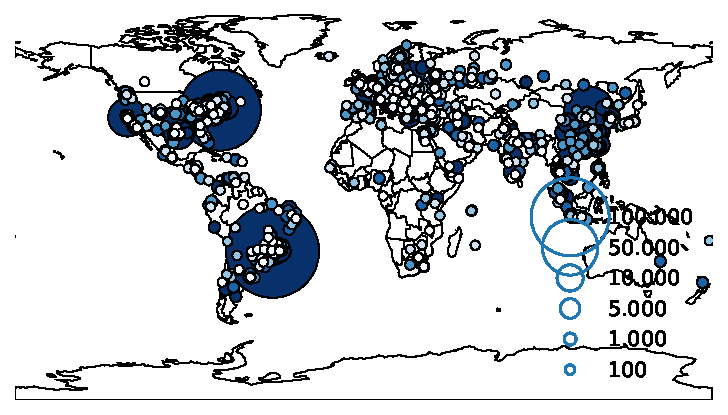
\includegraphics[width=\linewidth]{images/map_attack_locations.pdf}
    \caption{Number of received packets per location}
    \label{fig:map_attack_location}
\end{figure}

The honeypot received traffic from 126 unique countries. Table \ref{table:ip_locations} shows the top countries with incoming traffic. The table also shows the total size of the received packets, the number of unique IP addresses and number of unique Autonomous Systems the IP addresses belong to. As can be seen, the United States of America is the top country with 1.23 times as much traffic originated compared to the number two country, Brazil. When comparing this to the fifth country in terms of received packers, the Republic of Korea, there is almost 12.3 times less traffic compared to the United States of America.

\begin{table}[h]
\centering
\begin{tabular}{ |l|r|r|r|r| } 
\hline
Country & \# packets & size & \# IPs & \# ASNs \\ \hline
US & 230,147 & 22.2MB & 832 & 103 \\ \hline
BR & 186,300 & 17.4MB & 288 & 95 \\ \hline
CN & 115,463 & 12.1MB & 722 & 52 \\ \hline
RU & 19,400 & 1.5MB & 188 & 93 \\ \hline
KR & 18,847 & 1.7MB & 112 & 23 \\ \hline
\end{tabular}
\caption{Top attacker countries}
\label{table:ip_locations}
\end{table}

To understand why the United States, Brazil and China are the largest attacker countries we can take a look at which Autonomous Systems the IP addresses belong to. Traffic was received from a total of 1059 unique Autonomous Systems. Table \ref{table:asn_attacks} displays the top five Autonomous Systems from which most data has been received.

\begin{table}[h]
\centering
\begin{tabular}{ |l|l|r|r|r| } 
\hline
ASN & owner & \# packets & size & \# IPs \\ \hline
AS14061 & DigitalOcean & 175,820 & 17.4MB & 502 \\ \hline
AS8075 & Microsoft & 145,377 & 14.4MB & 16 \\ \hline
AS15169 & Google & 49,121 & 4,8MB & 150 \\ \hline
AS45090 & Tencent & 29,801 & 2.9MB & 42 \\ \hline
AS4134 & Chinanet & 29,422 & 3.6MB & 269 \\ \hline
\end{tabular}
\caption{Top attacker Autonomous Systems}
\label{table:asn_attacks}
\end{table}

Most of the largest subnets traffic has been received from are owned by large cloud providers from China, the United States of America and Brazil. This could also explain the large number of traffic received from these countries as cloud providers can offer capacity, affordability and flexibility. These systems are a common source for attacks as criminals often avoid paying for these systems by taking advantage of free services and trials or by hacking legitimate accounts for their attacks according to research by Akamai, an American Content Delivery Network (CDN) \cite{DDOSCSP:AKAMAI:2019}. This could be an explanation for the large number of traffic from these countries. As a sidenote, 97\% of the traffic from the Autonomous System from Microsoft originated from a single host.

To get a better understanding of when traffic was received and where the traffic originated from, the graph in Figure \ref{fig:data_time_continent} was created to display the amount of received data per continent for each period of 12 hours. This clearly shows a peak a few hours after creation of the honeypot, which displays the moment when the honeypot was discovered by automated systems from attackers. The hackers discover the open services at the IP, attempt to break into the router and after many unsuccessful attempts continue with other devices. The largest attacker at the first peak comes from the DigitalOcean Autonomous System. Another peak is at May 29, when one large large brute-force attacks was attempted from servers of Microsoft Azure in Brazil.

\begin{figure}[ht]
    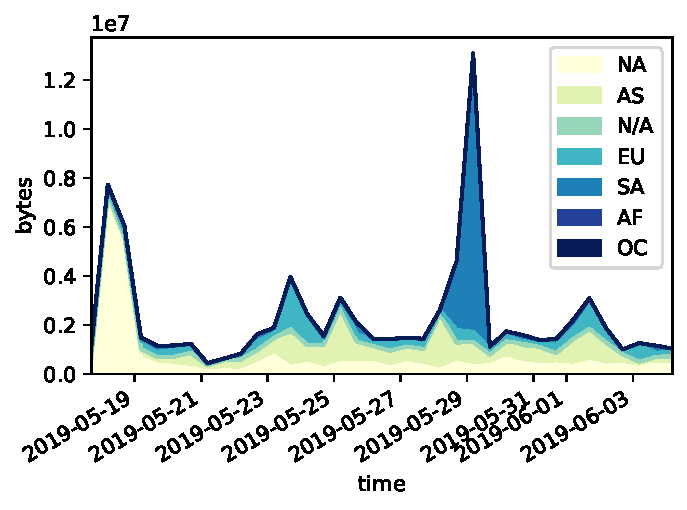
\includegraphics[width=\linewidth]{images/data_time_continent.pdf}
    \caption{Traffic received per continent for each 12 hour time period}
    \label{fig:data_time_continent}
\end{figure}

The top IP address has sent a total of 141,234 packets and 13.9MB of data and orginated from a Brazilian attacker from the Microsoft Azure ASN. The only other sending a similar amount of traffic is an attacker from the DigitalOcean ASN, which sent a total of 11.2MB. As displayed in Figure \ref{fig:ip_packet_cdf}, the number of packets per IP quickly declines, and more than half of the IP addresses never sent more than ten packets. Half of the data has been sent by only 55 IP addresses, which is 1.21\% of the total number of IP addresses. The top IP address has sent 23\% of the packets. The number of IP addresses in the graph has been displayed on a logarithmic scale for readability. 

\begin{figure}[ht]
    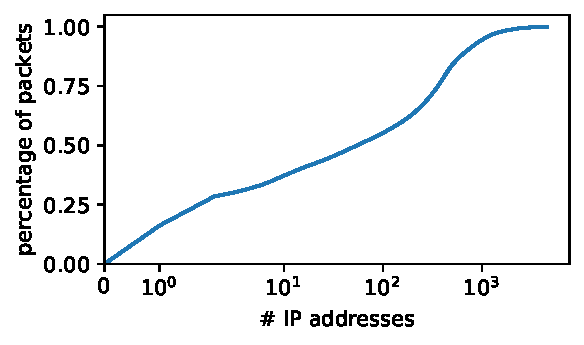
\includegraphics[width=\linewidth]{images/ip_packet_cdf.pdf}
    \caption{CDF of packets and IP addresses}
    \label{fig:ip_packet_cdf}
\end{figure}

Figure \ref{fig:dest_port_graph} shows the distribution of destination ports. Most traffic was targeted at the SSH server at port 22 and the Telnet server at port 23. Much less traffic was received at the web interface at port 80 and the WinBox port 8291. Almost no traffic was received on the SMB service on port 139, the MikroTik-bandwidth-test-server on port 2000 and the FTP server on port 21.

The SSH and Telnet server mostly received multiple large untargeted brute-force attacks trying many standard username and password combinations. Automating brute-force attacks for a common service such as SSH or Telnet is easier than targeting web interfaces on port 80 that differ between manufacturer and model. For this research the traffic on port 8291 is most relevant as this port is used to run the WinBox service and vulnerability CVE-2018-14847 is applicable to this port, therefore increasing the chance of receiving targeted attacks on this port. The low number of packets on port 139 could be an indicator that CVE-2018-7445 is not commonly exploited by attackers.

\begin{figure}[ht]
    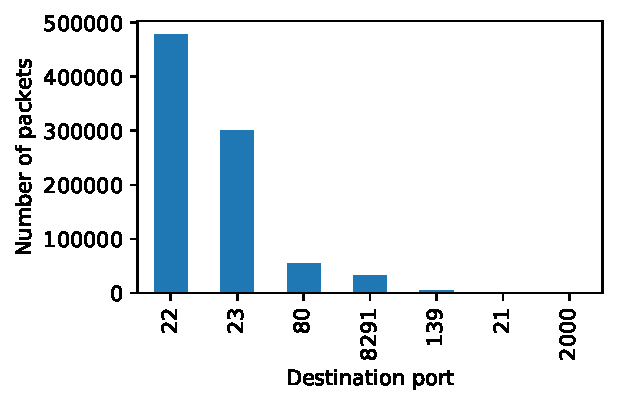
\includegraphics[width=\linewidth]{images/dest_port_packet_graph.pdf}
    \caption{Number of received packets per destination port}
    \label{fig:dest_port_graph}
\end{figure}

There is no clear pattern in the distribution of source ports, as the ports numbers are distributed evenly and the only 282 packets have been received from the top source port. Traffic has been received from a total of 32,788 unique source ports amounting to an average of only 27 received packets per source port.

\subsection{CVE-2018-14847}
The honeypot received large amounts of traffic targeting the critical vulnerability CVE-2018-14847. By filtering the traffic on the TCP streams containing containing one of the payloads, we discovered a total of 3,361 unique TCP streams, which combined amounts to 2.3\% of all in and outgoing traffic on the honeypot, which is quite a significant number considering most traffic is related to simple brute force attacks on the SSH and Telnet ports and that this vulnerability only applies to MikroTik devices. Comparing this to all traffic on port 8291, we can see that this is 71.1\% of all traffic on this port is related to CVE-2018-14847. All attacks targeting this vulnerability exploited this vulnerability to acquire the credentials of the administrator account, while none of the attackers used this vulnerability to enable a root shell on the router or for other purposes.

Around the same time period, other security researchers from GreyNoise Intelligence discovered a 6,700\% increase in attack and scan traffic on port 8291 targeting this vulnerability on their honeypots \cite{6700INC14847:TWITTER:2019}. This was discovered at June 12, eight days after the data capture for this research was halted. To discover if the data of this research supports a similar pattern a graph was made with traffic related to CVE-2018-14847 and the time, which is displayed in Figure \ref{fig:CVE-2018-14847-TRAFFIC}.

\begin{figure}[ht]
    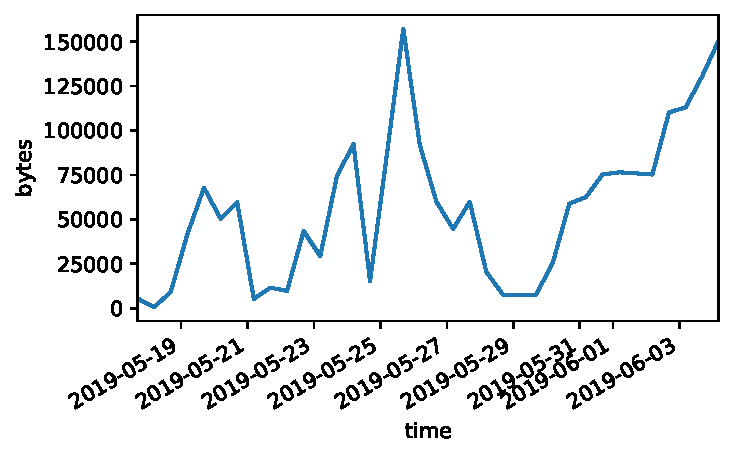
\includegraphics[width=\linewidth]{images/cve_14847_traffic.pdf}
    \caption{Traffic related to CVE-2018-14847 for each 12 hour time period}
    \label{fig:CVE-2018-14847-TRAFFIC}
\end{figure}

A spike in traffic related to CVE-2018-14847 can be seen around May 26 after which the traffic declines and after May 31 the traffic increases to approximately the same amount of traffic as the first spike. The biggest increase in traffic experienced is between the period of May 31 to June 4, which is an increase of 1,974\%. This increase is not close to the 6,700\% discovered by GreyNoise Intelligence. The increase was discovered eight days after the data capture for this research was finished. Therefore, this research does not have enough data to confirm or deny their statement. 

Table \ref{table:asn-cve-14847} shows the autonomous systems related to the attacks on CVE-2018-14847. Traffic was received from a total of 111 unique IP addresses and five Autonomous Systems. The top Autonomous System is the Google Cloud Platform (GCP) with attacks from 106 unique IP addresses originating there.

\begin{table}[h]
\centering
\begin{tabular}{ |l|l|r|r|r| } 
\hline
ASN & owner & \# packets & size & \# IPs \\ \hline
AS15169 & Google & 22,353 & 2.0MB & 106 \\ \hline
AS205544 & Leaseweb & 54 & 4.8KB & 2 \\ \hline
AS51167 & Cantabo & 14 & 1.2KB & 1 \\ \hline
AS42387 & Svyazservice & 8 & 641b & 1 \\ \hline
AS62403 & Disk Group & 7 & 637b & 1 \\ \hline
\end{tabular}
\caption{CVE-2018-14847 Autonomous Systems}
\label{table:asn-cve-14847}
\end{table}

The Google Autonomous System includes the BGP ranges belonging to the Google Cloud Platform. To understand why nearly all attackers for CVE-2018-14847 chose to use the Google Cloud Platform, we decided to examine the offerings of the Google Cloud Platform. As research by the security company Akamai showed, criminals often avoid paying by either taking advantage of free trials or by hijacking legitimate accounts. For this reason, we decided to look if the Google Cloud Platform offers free trials or service or if it is more competitive than either Microsoft Azure or Amazon Web Services.

The Google Cloud Platform offers one basic virtual machine per month\footnote{See: \url{https://cloud.google.com/free/} (18 June 2019)} with no time limit. The competitor, Amazon Web Services has a free tier with a free virtual machine with a 750 hour limit\footnote{See: \url{https://aws.amazon.com/free} (19 June 2019)} and Microsoft Azure offers a similar free virtual machine with a 750 hour limit \footnote{See: \url{https://azure.microsoft.com/free/} (19 June 2019)}. Furthermore, the Google Cloud Platform offers a free Google Cloud Shell to anyone owning a Google account, providing attackers access to a complete Linux virtual machine accessible from a web browser with root capabilities and few limitations\footnote{See: \url{https://cloud.google.com/shell/} (18 June 2019)}. For this type of attack, it could be that Google Cloud Platform is more popular by attackers than the free services of the competitors, because it provides the free virtual machines and the Cloud Shell.

\subsection{DNS redirection}
The honeypot experienced a significant number of DNS redirection attempts. All of these attempts were received on port 80 and 8291. Of this traffic, 55.3\% of these on port 80 and the other 44.7\% on port 8291. Most of these attempts originated from the same hosts as the attacks targeting CVE-2018-14847. At least some of these attacks were successful, as some attackers succeeded in updating the DNS servers on the router to servers hosted in the Google Cloud Plaform. The attackers exploited the CVE-2018-14847 vulnerability to acquire the user database. This database was then decrypted to retrieve the credentials of the administrator account and the attacker continued by signing in to the router management interface to update the DNS settings.

The traffic related to DNS redirection attacks is 1.5\% of the traffic, excluding the 2.3\% related to CVE-2018-14847. By splitting this up per port we can see that 21.0\% of all traffic on port 8291 is related to DNS redirection attacks and 23.3\% of all traffic on port 80. Of the 2.3\% five different types of untargeted attacks were discovered, targeting D-Link, ARG, DSLink, Secutech and TOTOLINK routers \cite{DLINK:DNSHIJACK:2019}. Table \ref{table:dns_redirection_requests} shows the different brands with the number of observed requests and the request itself.

\begin{table}[h]
\centering
\begin{tabular}{ |l|l|l| } 
\hline
Brand & count & DNS redirection request \\ \hline
ARG & 393 & /form2dns.cgi?dnsmode=1?...\\ \hline
D-Link & 785 & /dnscfg.cgi?dnsPrimary=...\\ \hline
DSLINK & 393 & /action?dns\_status=1...\\ \hline
Secutech & 785 & /wan\_dns.asp?go=...\\ \hline
TOTOLINK & 393 & /boafrm/formbasesetcpipsetup.. \\ \hline
\end{tabular}
\caption{Number of DNS redirection attacks per router brand}
\label{table:dns_redirection_requests}
\end{table}

All requests were observed at least 393 times, with only the TOTOLINK and Secutech being targeted almost twice. By digging further in the traffic we observed a pattern where in each attack, except for one, an attacker sent one request for the TOTOLINK, DSLINK and ARG routers and two requests for the Secutech and D-Link routers. The attacks on port 8291 were usually followed by traffic related to CVE-2018-14847 from the same hosts. This specific characteristic is an indicator that the DNS redirection attacks and the attacks exploiting CVE-2018-14847 could be coming from one or a small group of attackers. Another argument pointing in this direction is that all of the 82 IP addresses performing this attack and nearly all of the traffic related to CVE-2018-14847 originates from the Google Cloud Platform and there is a large overlap in IP addresses related to the DNS redirection attacks and the CVE-2018-14847 vulnerability.

By looking at the IP addresses of the DNS servers included in the requests, five different waves of attacks were discovered, each with a different rogue DNS server. The first of these rogue DNS servers was hosted in Microsoft Azure and the other four were hosted in the Google Cloud Platform. These five DNS servers filtered the incoming DNS requests, making it difficult to discover the intent of the attackers.

\subsection{Point-to-Point Tunneling Protocol}
Another attack that was discovered on the honeypot is a single attack by an attacker from Palestine. The attacker managed to sign in to the system via the WinBox program on port 8291. The logging entries in Table \ref{table:pptp_attack_log} show that the attacker signed in via the WinBox program to change the Point-to-Point Tunneling Protocol (PPTP) settings with the intent of setting up a tunneled connection to the outside. This is a targeted attack, since the user accounts have a strong password and no successful brute-force attempt has been discovered. There is no other traffic from this Palestinian IP, so it cannot be confirmed what method was used by the attacker to acquire the administrator credentials. CVE-2018-14847 is the most likely vulnerability, as this vulnerability has been confirmed to be used by other attackers to retrieve the administrator credentials.

\begin{table}[h]
\centering
\begin{tabular}{ |l|l| } 
\hline
time & message \\ \hline
01:49:59 & user admin logged in from <ip> via winbox \\ \hline
01:50:07 & PPTP Server settings changed by admin \\ \hline
01:50:52 & ppp profile <default> changed by admin \\ \hline
01:51:08 & ppp secret <ppp1> added by admin \\ \hline
01:51:09 & user admin logged out from <ip> via winbox \\ \hline
\end{tabular}
\caption{Log messages for the PPTP attack}
\label{table:pptp_attack_log}
\end{table}

\subsection{IoT Malware}
The honeypot did receive a lot of traffic related to IoT Malware. The total traffic was filtered to discover if there is any traffic related to the Mirai malware, as there is a filter available to detect traffic related to Mirai \cite{IMPROVINGIOTBOTNET:SENSORS:2018}. From this we discovered that a total of 1.0\% of the traffic is related to Mirai, which is a total of 8091 incoming and outgoing packets. Of the traffic, 95.4\% was targeted at the Telnet server on port 23, 4.1\% targeted the SSH server at port 22 and 0.5\% targeted the web service at port 80.

All traffic related to Mirai can be characterized by connecting and after an ACK packet has been received resetting the connection by sending a packet with the RST flag. Of the Mirai traffic, 19.5\% of the packets are RST packets. The server receiving the packet usually then responds with TCP Retransmission packets, which is 41.8\% of the Mirai related packets. There were a total of unique 2212 IP addresses, which is 48.5\% of all the IP addresses.

Most of the vulnerable devices can be attributed to three Chinese Autonomous System: Hi-Net, Chinanet and the CNCGroup, which combined have 25.3\% of all the infected devices from which traffic has been received. Other large Autonomous Systems include TE-AS from Egypt, Rostelecom from Russia and IBSNAZ from Italy. The first infected cloud provider is Digital Ocean with 168 infected IP addresses. Mirai mostly targets vulnerable Internet of Things devices, such as IP cameras \cite{UNDERSTANDINGMIRAI:USENIX:2017} and for this reason most of the Mirai related traffic has been received from local Internet Service Providers (ISPs) and not from cloud services.

\subsection{Denial-of-Service}
During the phase of data capture with the honeypot, we discovered that the honeypot sometimes rebooted multiple times per day and in some cases a few times per hour. By looking at the logs, many of these reboots could be confirmed, but not all of them. This is because the logs only capture the current information every five minutes and the logs were not able to be retrieved every time. After May 20 on 22:15 CEST no log data is available. This is after an attacker entered the system and changed the DNS and the PPTP settings to an IP address of one of the rogue DNS servers from the DNS redirection attempts. After the attack the router closed off all incoming TCP connections by responding with a FIN packet. This stopped on May 22 14:40 CEST when the DNS server was discovered and removed from the DNS settings. Since then the traffic continued like normal. Due to this attack the live diagnostics script was unable to retrieve any log file from the router during that period.

A total of 71 reboots could be confirmed from the logs. When the router reboots, the logs are cleared and a log entry is added showing the time of reboot. As mentioned before, the number of reboots is estimated to be higher as no data is available for May 21 and the logs are only captured every five minutes. The last observed reboot was at May 23 at 15:34 CEST. Just after that time, we updated the Simple Network Management Protocol (SNMP) configuration and enabled Universal Plug and Play (UPnP). After these changes, no reboot has been observed. In Figure \ref{fig:observered_reboots} the number of confirmed reboots is displayed for the period between May 17 and May 25.

\begin{figure}[ht]
    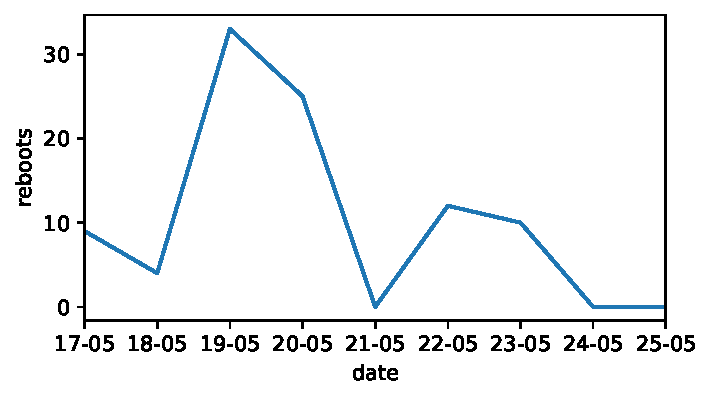
\includegraphics[width=\linewidth]{images/reboots_plot.pdf}
    \caption{Number of confirmed reboots per day}
    \label{fig:observered_reboots}
\end{figure}

To get a better understanding of the cause of the reboots, the logs were compared with the network traffic. Most of the time, the reboot occured after one or multiple RST packet was received from a device infected with the Mirai malware. This is similar to CVE-2017-7285, as in this vulnerability the router is prevented the router from establishing new TCP connections after a flood of RST packets is received \cite{CVE-2017-7285:CXSECURIITY:2017}. The main difference between this attack and CVE-2017-7285 is that CVE-2017-7285 is not confirmed to cause reboots and CVE-201707285 has already been patched in the release of RouterOS used in the honeypot. For these reasons it is unlikely that these reboots are caused by CVE-2017-7285, although a similar vulnerability might be the cause of the observed reboots.
\section{Conclusion}
In this paper, attacks on low-cost routers were characterized by using a honeypot router to capture real hacker attacks. The paper discussed some common attacks targeting low-cost routers, such as DNS redirection attacks and code injection attacks. The honeypot router RouterOS from MikroTik was used, since RouterOS is a common vendor providing low-cost routers and in recent years multiple critical vulnerabilities were published for RouterOS. The honeypot was designed with the five principles for a secure honeypot in mind \cite{HONEYPOTSLIABILITY:SPRINGER:2015} and during the deployment of the honeypot all traffic and log files were captured.

With this approach, multiple different attacks were discovered. CVE-2018-14847 was the most common vulnerability targeted by attackers and was used to acquire the administrator credentials. These credentials were used to manually sign in and update the DNS server. Of all traffic on RouterOS specific port 8291, 71.1\% was related to this vulnerability. The attacks on CVE-2018-14847 were usually combined with untargeted DNS redirection attempts, which were 21.0\% of all traffic on port 8291 and 23.3\% of all traffic on the web interface at port 80. These DNS redirection attempts all originated from the Google Cloud Platform and followed the same characteristics. The other attacks include traffic from Internet of Things malware and a hacker updating the PPTP settings in the router. Furthermore, it was discovered that the router rebooted multiple times, usually after receiving one or multiple RST packets. 

The intents of the attackers could be characterized by either aiming to redirect traffic (DNS redirection / CVE-2018-14847), to intercept traffic (PPTP) or to deny traffic to the router (DoS / IoT Malware), with nearly all of the targeted attacks originating in cloud services.

\section{Discussion and Future work}
In this research, only attacks on low-cost routers from MikroTik were analyzed. In future research, honeypots simulating other brands of low-cost routers could be used to discover if there are differences in the characteristics of attacks between multiple vendors. Since this research was done by capturing attacks with a single honeypot in Brazil, more honeypots could be used per type of vendor and placed in different regions in order to detect regional differences in the discovered attacks.

Another improvement for future work could be to capture data for a longer period of time. This research was limited by the amount of research credits provided by Microsoft Azure, which limited the data capture to a short period of time. By collecting data for a longer period, it would become easier to discover patterns or trends in the observed attacks.


\balance

%ACKNOWLEDGMENTS are optional
% \section{Acknowledgments}

% The following two commands are all you need in the
% initial runs of your .tex file to
% produce the bibliography for the citations in your paper.
\bibliographystyle{ieeetr}
\bibliography{sigproc}  % sigproc.bib is the name of the Bibliography in this case
% You must have a proper ".bib" file
%  and remember to run:
% latex bibtex latex latex
% to resolve all references
%
% ACM needs 'a single self-contained file'!
%
% \vspace{50 mm}
% \newpage
%APPENDICES are optional
% \appendix
% Appendix A
% \section{Headings in Appendices}
% The rules about hierarchical headings discussed above for the body
% of the article are different in the appendices. In the
% \textbf{appendix} environment, the command \textbf{section} is
% used to indicate the start of each Appendix, with alphabetic order
% designation (i.e. the first is A, the second B, etc.) and a title
% (if you include one).  So, if you need hierarchical structure
% \textit{within} an Appendix, start with \textbf{subsection} as the
% highest level. Here is an outline of the body of this document in
% Appendix-appropriate form:
% \subsection{Introduction}
% \subsection{The Body of the Paper}
% \subsubsection{Type Changes and  Special Characters}
% \subsubsection{Math Equations}
% \paragraph{Inline (In-text) Equations}
% \paragraph{Display Equations}
% \subsubsection{Citations}
% \subsubsection{Tables}
% \subsubsection{Figures}
% \subsubsection{Theorem-like Constructs}
% \subsubsection*{A Caveat for the \TeX\ Expert}
% \subsection{Conclusions}
% \subsection{Acknowledgments}
% \subsection{Additional Authors}
% This section is inserted by \LaTeX; you do not insert it. You just
% add the names and information in the
% \texttt{{\char'134}additionalauthors} command at the start of the
% document.
% \subsection{References}
% Generated by bibtex from your ~.bib file.  Run latex, then bibtex,
% then latex twice (to resolve references) to create the ~.bbl file.
% Insert that ~.bbl file into the .tex source file and comment out
% the command \texttt{{\char'134}thebibliography}.
% % This next section command marks the start of
% % Appendix B, and does not continue the present hierarchy
% \section{More Help for the Hardy}
% The sig-alternate.cls file itself is chock-full of succinct and
% helpful comments.  If you consider yourself a moderately
% experienced to expert user of \LaTeX, you may find reading it
% useful but please remember not to change it.
%\balancecolumns % GM June 2007
% That's all folks!

% \balancecolumns
\end{document}